\chapter{A brief tour of Monteverdi}\label{chap:Monteverdi} 

\section{Introduction}\label{sec:montintro}
The \app package makes available a set of simple software
tools which were designed to demonstrates what can be done with
\otb. Many users started using these applications for real processing
tasks, so we tried to make them more generic, more robust and easy to
use. \otb users have been asking for an integrated application for a
while, since using several applications for a complete processing
(ortho-rectification, segmentation, classification, etc.) can be a
burden. Recently, the OTB team received a request from CNES' Strategy
and Programs Office in order to provide an integrated application for
capacity building activities (teaching, simple image manipulation,
etc.). The specifications included ease of integration of new
processing modules.  

\section{Installation}\label{sec:montinstall} 
The application is called \mont, since this is the name of the Orfeo
composer.The application allows you to build interactivelly remote
sensing processes based on the \otb. This is also in
rembering of the great (and once open source) Khoros/Cantata
software.  Installation of \mont is very simple. Standard
installer packages are available on MS Windows and MacOS X.  For many
flavors of GNU/Linux binary packages (rpm and deb) or software
repositories to add to your installation manager are also provided. 
Get the latest information on binary packages on the \website.

\section{Anatomy of the applications}\label{sec:anatomy}

\subsection{What does it look like?}

\begin{figure}
  \center
  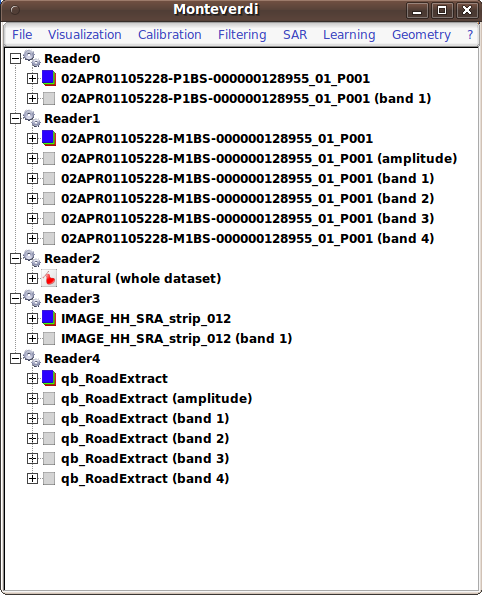
\includegraphics[width=0.6\textwidth]{../Art/MonteverdiImages/monteverdi_mainwindow.png}
  \itkcaption[Monteverdi main window]{Monteverdi main window.}
  \label{fig:mainwindow}
\end{figure}

This is Monteverdi's main window (figure ~\ref{fig:mainwindow} )where the
menus are available and where you can see the different modules which
have been set up for the processing. Input data are obtained by
readers. When you choose to use a new module, you select its input
data, and therefore, you build a processing pipeline sequentially.
Figure ~\ref{fig:inputswindow} shows the generic window which allows to
specify output(s) of Monteverdi's modules.  

\begin{figure} 
  \center
  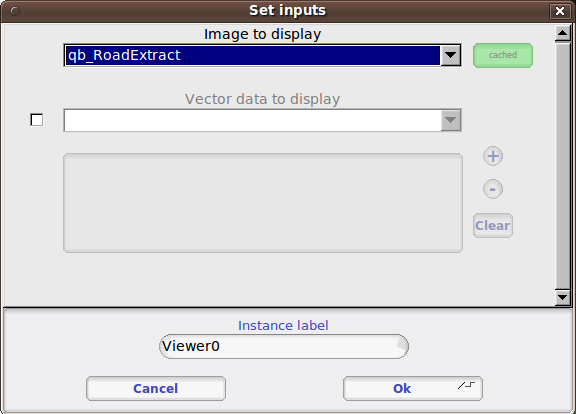
\includegraphics[width=0.6\textwidth]{../Art/MonteverdiImages/monteverdi_inputs_window.png}
  \itkcaption[Monteverdi main window]{Monteverdi inputs selection
    generic window.}  \label{fig:inputswindow} 
\end{figure} 

Let's have a look at the different menus. The first one is of course
the "File" menu. This menu allows you to open a data set, to save it
and to cache it. The "data set" concept is interesting, since you
don't need to define by hand if you are looking for an image or a
vector file. Of course, you don't need to do anything special for any
particular file format. So opening a data set will create a "reader"
which will appear in the main window. At any time, you can use the
"save data set" option in order to store to a file the result of any
processing module.


\subsection{Open an image with \mont}
The application allows to interactively select raster/vector dataset
by browsing your computer. Monteverdi takes advantage of the automatic
detection of images' extensions to indicate the dataset type (optical,
SAR or vector data).

The input dataset is added to the "Data and Process" tree whcich
describes the dataset content and each node corresponds to a layer.

\subsection{Visualize an image with \mont}
This module allows to visualize raster or vector data. It allows to
create RGB composition from the imput rasters. It is also possible to
add vector dataset which are automatically reproject in the same
projection of the input image or Digital Elevation informations.

The viewer offers three types of data visualisation: 

\begin{itemize}
\item The scroll Window : to navigate quickly inside the entire scene
\item The Full resolution window: the view of the region of interest
  selected in the scroll window
\item The Zoom window
\item The Pixel description: give access to dynamic informations on
  the current pixel pointed. Informations display are:
  \begin{itemize}
  \item The current index
  \item The pixel value 
  \item The computed value (the dynamic of hte input image is modify
    to get a proper visualisation
  \item The coordinates of the current pixel (longitude and latitude)
  \item In case where there is a Internet connection available,
    Monteverdi displays the estimate location of the current pixel
    (country + city)
  \end{itemize} 
\end{itemize}

\begin{figure} 
  \center
  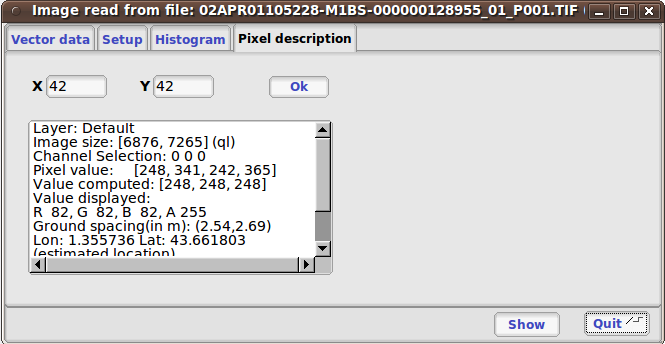
\includegraphics[width=0.6\textwidth]{../Art/MonteverdiImages/monteverdi_viewer_pixel_description.png}
  \itkcaption[Monteverdi main window]{Monteverdi pixel description box.}
  \label{fig:viewerpixeldescription}
\end{figure}

The Visualization offers others great functionnalities which are
available in the detached window.  It is for example possible to
superpose vector dataset to the input image (see figure
~\ref{fig:viewervectordata}).

\begin{figure}
  \center
  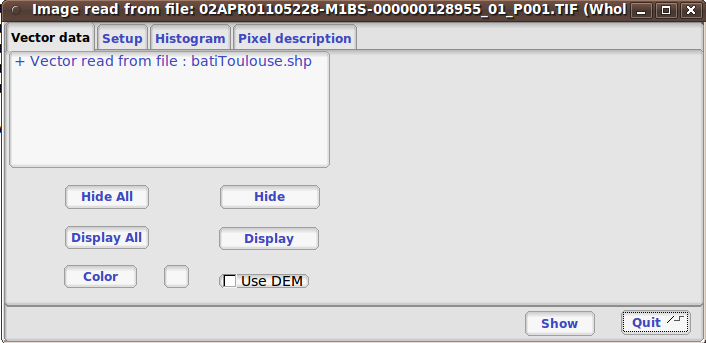
\includegraphics[width=0.6\textwidth]{../Art/MonteverdiImages/monteverdi_viewer_vector_data.png}
  \itkcaption[Vector Data visualization]{Monteverdi pixel description box.}
  \label{fig:viewervectordata}
\end{figure}

The "Setup Tab" allow to modify the RGB composition or use the
grayscale mode to display only one layer.

\begin{figure}
  \center
  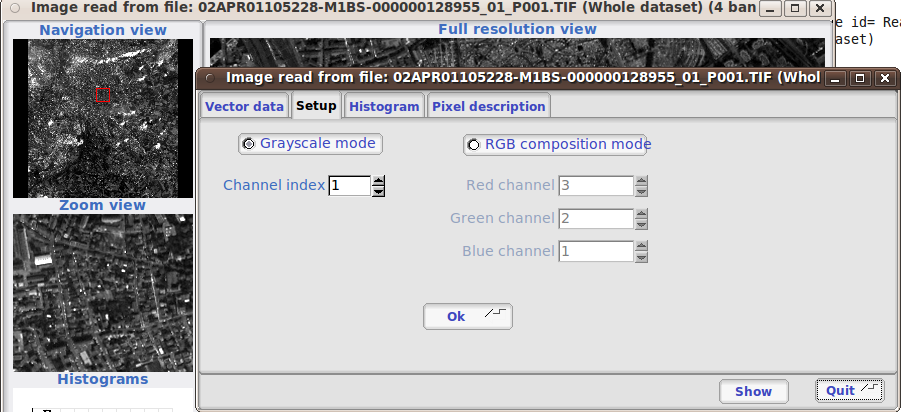
\includegraphics[width=0.6\textwidth]{../Art/MonteverdiImages/monteverdi_viewer_rgb_composition.png}
  \itkcaption[Manage RGB composition]{Manage RGB composition.}
  \label{fig:rgbcomposition}
\end{figure}

The "Histogram Tab" get access to the dynamic of the displayed
layers. The basic idea is to convert the output of the pixel
representation to a RGB pixel for rendering on conventional displays.
Values are contrained to 0-255 with a transfer function and a clamping
operation.  By default, the dynamic of each layer is modified by
clamping the histogram at $min + 2\%$ and $max - 2\%$.

\begin{figure}
  \center
  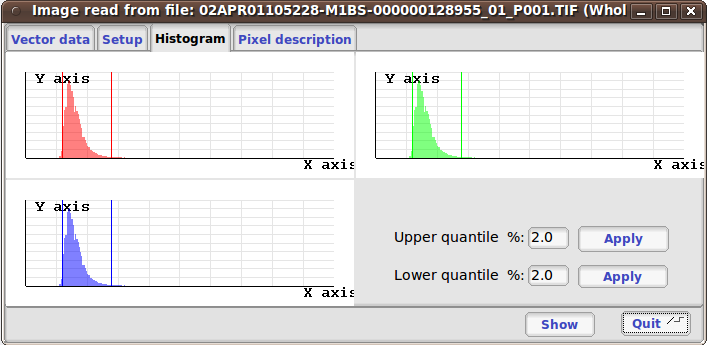
\includegraphics[width=0.6\textwidth]{../Art/MonteverdiImages/monteverdi_viewer_histogram.png}
  \itkcaption[Manage the dynamic of each layer]{Manage the dynamic.}
  \label{fig:histogram}
\end{figure}

There is also possible to select pixel coordinates and get access to all the informations abvailable in the ``Pixel description 
Box''.

\begin{figure}
  \center
  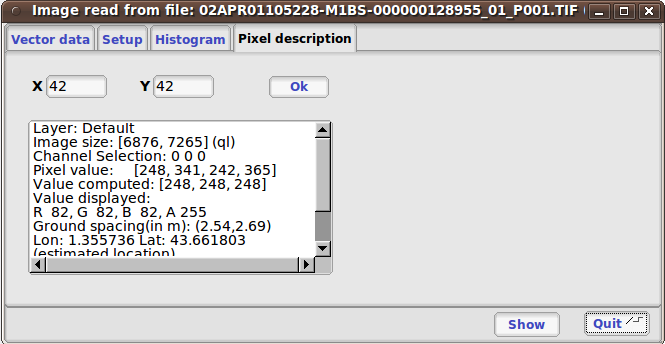
\includegraphics[width=0.6\textwidth]{../Art/MonteverdiImages/monteverdi_viewer_pixel_description.png}
  \itkcaption[Pixel description via index selection]{Index description via index selection.}
  \label{fig:pixeldescriptioninformations}
\end{figure}

\subsection{Cache dataset}
The "cache data set" (see figure ~\ref{fig:cachingmodule}) is a very
interesting functionality. As you know, OTB implements processing on
demand, so when you build a processing pipeline, no processing takes
place unless you ask for it explicitly. That means that you can plug
together the opening of a data set, an orthorectification and a
spleckle filter, for example, but nothing will really be computed
until you trigger the pipeline execution. This is very convenient,
since you can quickly build a processing pipeline and let it execute
afterwards while you have a coffee. In \mont, the process is executed
by saving the result of the last module of a pipeline. However,
sometimes, you may want to execute a part of the pipeline without
having to set the file name to the obtained result. You can do this by
caching a data set. That is, the result will be stored in a temporary
file which will be created in the "Caching" directory created by the
application. Another situation in which you may need to cache a data
set is when you need that the input of a module exists when you set
its parameters. This is nor a real requirement, since Monteverdi will
generate the needed data by streaming it, but this can be
inefficient. This for instance about visualization of the result of a
complex processing. Using streaming for browsing through the result
image means processing the visible part every time you move inside the
image. Caching the data before visualization will generate the whole
data set in advance allowing for a more swift display. All modules
allow you to cache their input data sets.

\begin{figure}
  \center
  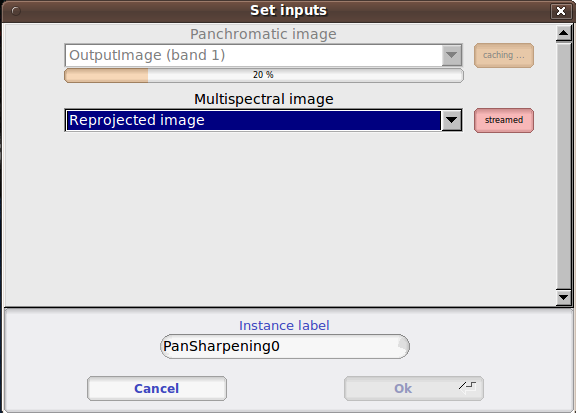
\includegraphics[width=0.6\textwidth]{../Art/MonteverdiImages/monteverdi_caching_module.png}
  \itkcaption[Cache operation on the panchromatic image in progress]{Cached and streamed dataset.}
  \label{fig:cachingmodule}
\end{figure}

%Section describing the monteverdi architecture of the application (perhap's not relevant in the cookbook)

\subsection{Dynamic GUI definition}
The aim of \mont is to provide a generic interface which is based on
the definition of the internal processes.  In this frame, the way that
that you have to manage modules are identical during the definition of
a new process.  Selecting a module on the upper main window, open
automatically the "Inputs definition Window" wich allows to select
data which are inputs of the current module. \mont module can manage
single or multiple inputs and these inputs can be images on your
computer or results of previous module already registered in the "Data
and Process" tree.
    
\subsection{Dynamic I/O definition}
Management of image formats in \mont works in the same manner as in
the \otb.  The principle is that the software automatically recognize
the image format.  Communication between modules follow also the same
principle and the Input definition of modules request to all available
outputs of the same type in the "Data and process" tree.  Internally,
all the treatments in \mont are computed in float precision by
default. It is also possible to switch to double precision by
compiling the application from source and set the CMAKE option compile
float to ON.

%Section describing some available modules in the application
\section{Available modules}\label{sec:modules} 
\subsection{I/O operations}
\subsubsection{Extract region of interest}
It allows to extract regions of interest (ROI) from an image. There
are two ways to select the region:
\begin{itemize}
\item By indicating the X and Y coordinatres of the upper-left
  coordinates and the X-Y size of the regions.
\item By interactivelly selecting the region of interest in the input image.
\end{itemize}

\subsubsection{Concatenate image bands}
With \mont, you could generate a large scale of value added
informations from lots of inputs data. One of the basic functionnality
is to be able to superpose result's layers into the same dataset.
Concatenating images into one single multiple-bands image (they need
to have the same size), and to be able to create for example RGB
composition with the inputs layer.

\begin{figure}
  \center
  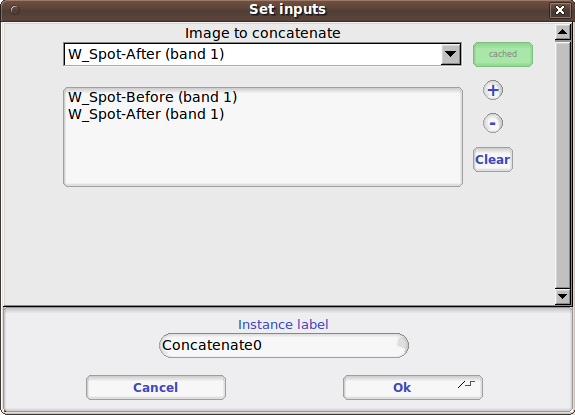
\includegraphics[width=0.6\textwidth]{../Art/MonteverdiImages/monteverdi_concatenate_before_after.png}
  \itkcaption[Concatenation of multitemporal data]{Concatenation module.}
  \label{fig:concatenate}
\end{figure}

\subsubsection{Save dataset to file}

\mont allows to export raster or vector dataset to a file to your
system.  In the case of raster images, it is possible to cast output
pixel type. In \mont all the processes are done in floating point
precision.  On large remote sensing dateset, saving your result in
float data type could lead to file too large(more than 25 Go for
pas-sharpened 8 bands WorldView2 with a resolution of $46$
centimeters). Since the module allows to cast pixels in other types :

\begin{itemize}
\item unsigned char (8 bits) 
\item short (16 bits)
\item int (32 bits)
\item float (32 bits)
\item double(64 bits)
\item unsigned short (16 bits)
\item unsigned int (32 bits)
\end{itemize}

\begin{figure}
  \center
  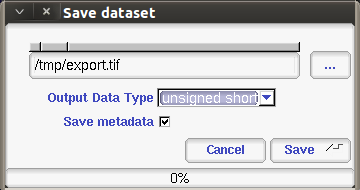
\includegraphics[width=0.6\textwidth]{../Art/MonteverdiImages/monteverdi_export_dataset.png}
  \itkcaption[Export dataset]{Save dataset module.}
  \label{fig:concatenate}
\end{figure}

\subsection{Geometric process}
In the frame of remote sensing process, one common operation is to be
able to superpose and manipulate data which come from different
sources.  This section gives access to a large set of geometric
operations.  It performs re-projection and orthorectification
operations on Optical or SAR dataset using the available sensor models
(image informations available in the meta-data are automatically read
by the application).  
\subsubsection{Reprojection module}
The application is derived from the otbOrthorectificationApplication
in the \app package and allow to produce orthorectified imagery from
level 1 product. The application is able to parse metadata
informations and set default parameters. The application contains 4
tabs:

\begin{itemize}
\item Coordinates: Define the center or upper-left pixel coordinates
  of the orthorectified image (the longitude and latitude coordinates
  are calculated through meta-data informations. It is also possible
  to specify the map projection of the output.
\item Output image: The module allow to only orthorectified a Region
  Of interest inside the input dataset. This tab allow to set the size
  of the ReOI around the center pixel coordinate or from the upper
  left index. The orthorectified imagery can also be resample at any
  resolution in the line or column directions by setting the "Spacing
  X" and the "Spacing Y" and choosing the method of interpolation.
\item DEM: Indicate path to a directory containing SRTM elevation
  file. The application is able to detect inside the direcory which
  DEM files are relevant in the process. You can find detailed
  informations on how to get a usable DEM
\item Image extent: Compare the initial image extension with the
  preview the orthorectified result. This preview is automatically
  updated if the user change the "Size X" or "Size Y" values in the
  "Output Image" tab.
\end{itemize}

\begin{figure}
  \center
  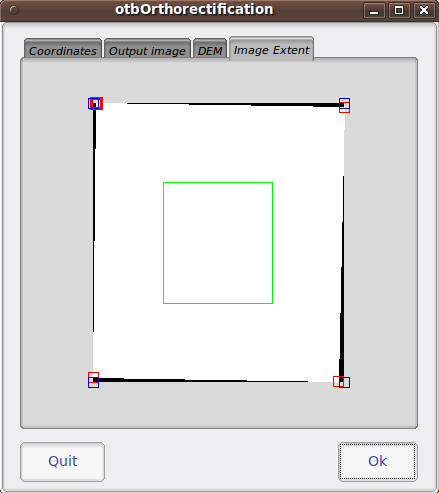
\includegraphics[width=0.6\textwidth]{../Art/MonteverdiImages/monteverdi_ortho_extent.png}
  \itkcaption[Preview of the orthorectified imagery]{Reprojection module.}
  \label{fig:ortho}
\end{figure}


\subsubsection{Estimating sensor model based on ground control points}
This module allows to take ground control points on a raster image
where no geographic informations are available.  This GCPs list is
making correspondence between pixel coordinate in the input image and
physical coordinates. The list allows to derive a general function
which to translate any pixel coordinates in physical positions. This
function is based on a RPC transformation (Rational Polynomial
Coefficients). As a consequence, the module enriches the output image
with metadata informations defining a RPC sensor model associated with
the input raster.  There is several ways to generate the GCPs:

\begin{itemize}
\item With Internet access: dynamically generate the correspondance on
  the input image and Open Street Map layers
\item Without Internet access: Set manually Ground control points :
  indicate index position and cartographic coordinates in the input
  image.
\end{itemize}

It is also possible to import/export the list of Ground Control points
from/to an XML file.

Moreover, if the input image have already GCPs in its metadata, the
module allows to add or remove points from the existing list which is
automatically loaded.

\subsection{Calibration}
In the solar spectrum, sensors on Earth remote sensing satellites
measure the radiance reflected by the atmosphere-Earth surface system
illuminated by the sun. This signal depends on the surface
reflectance, but it is also perturbed by two atmospheric processes,
the gaseous absorption and the scattering by molecules and aerosols.


\subsubsection{Optical calibration}
In the case of the Optical calibration, the basic idea is to be able
to retrieve reflectance of the observed physical object.  The input
image contains only numerical which The process can be split in 3 main
operations:
\begin{itemize}
\item Derived luminance from the raw value in the input image. 
\item Convert the Luminance to Reflectance to produce the TOA
  image(Top Of Atmosphere).
\item Inverse a radiative transfer code which simulate the reflection
  of solar radiation by a coupled atmosphere-surface system. This step
  produce the TOC (Top of Canopy) imagery which is the final result of
  the Optical calibration module.
\end{itemize}

\begin{figure}
  \center
  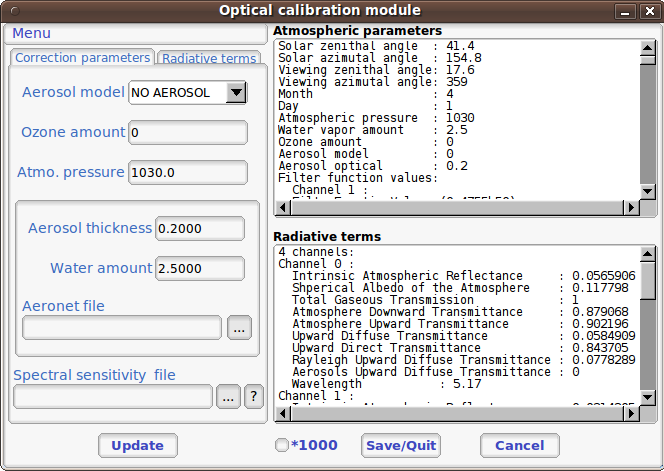
\includegraphics[width=0.6\textwidth]{../Art/MonteverdiImages/monteverdi_optical_calibration.png}
  \itkcaption[GUI of the optical calibration module based on the 6S model]{Optical calibration module.}
  \label{fig:opticalcalibration}
\end{figure}

The 6S model needs atmospheric parameters to be able to compute
radiative terms to estimate the atmoshperic contributions on the input
signal. Default parameters are available in the module but it is
possible to indicate AERONET file. The AERONET (AErosol RObotic
NETwork) program is a federation of ground-based remote sensing
aerosol networks established by NASA and PHOTONS (Univ. of Lille 1,
CNES, and CNRS-INSU) and is greatly expanded by collaborators from
national agencies, institutes, universities, individual scientists,
and partners. The program provides accessible public domain database
of aerosol optical, mircrophysical and radiative properties.

The module produce different outputs:

\begin{itemize}
\item Luminance image
\item TOA reflectance image
\item TOC reflectance image
\end{itemize}


\begin{figure}
  \center
  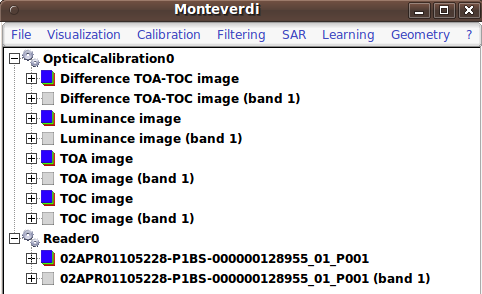
\includegraphics[width=0.6\textwidth]{../Art/MonteverdiImages/monteverdi_optical_calibration_outputs.png}
  \itkcaption[Output of the optical calibration module]{Optical calibration module's outputs.}
  \label{fig:opticalcalibrationoutput}
\end{figure}

\subsubsection{SAR calibration}

The calibration and validation of the measurement systems are
important to maintain the reliability and reproducibility of the SAR
measurements but the establishment of correspondence between
quantities measured by SAR and physical measure which requires
scientific background. The SAR calibration module allow to estimate
quantitative accuracy For now only calibration of TerraSARX data is
available.
%//TODO add description of outputs

\subsection{Filtering Operations}
\subsubsection{Band Math}
The Band Math module allows to perform complex mathematical operations
over images.It is based on the mathematical parser library muParser
and comes with a bunch of build-in functions and operators (listed
\href{http://muparser.sourceforge.net/mup_features.html#idDef2}{here}). This
homebrewed digital calculator is also bundled with custom functions
allowing to compute a full expression result simply and really fast,
since the filter supports streaming and multi-threading.  The \mont
module provides a intuitive way to perform complex band computation
the easy way. The module also prevents error in the mathematical
command by checking the expression as the user types it, and notifying
information on the detected error:

Figure ~ref{fig:bandmathndvi} presents an example on how the band math
can produce a threshold image on the NDVI value computed in one pass
using built-in conditional operator ``if'' available in the parser.

An other operational
example, on how this simple module can produce reliable information.
Figure ~\ref{fig:ndwi2} shows the result of the subtraction of the Water
indice on 2 images which was taken before and during the crisis event.
The difference was produce by the band math module and allow to get a
reliable estimation of the flood events.

\begin{figure}
  \center
  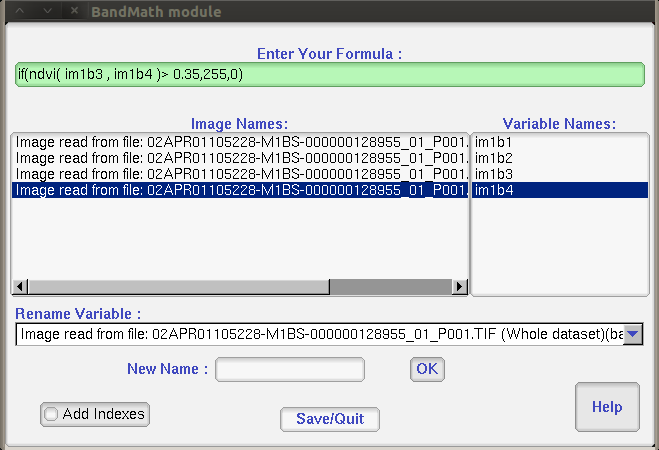
\includegraphics[width=0.6\textwidth]{../Art/MonteverdiImages/monteverdi_band_math_ndvi_threshold.png}
  \itkcaption[Band math module]{Conditional operators using the band math module.}
  \label{fig:bandmathndvi}
\end{figure}

\begin{figure}
  \center
  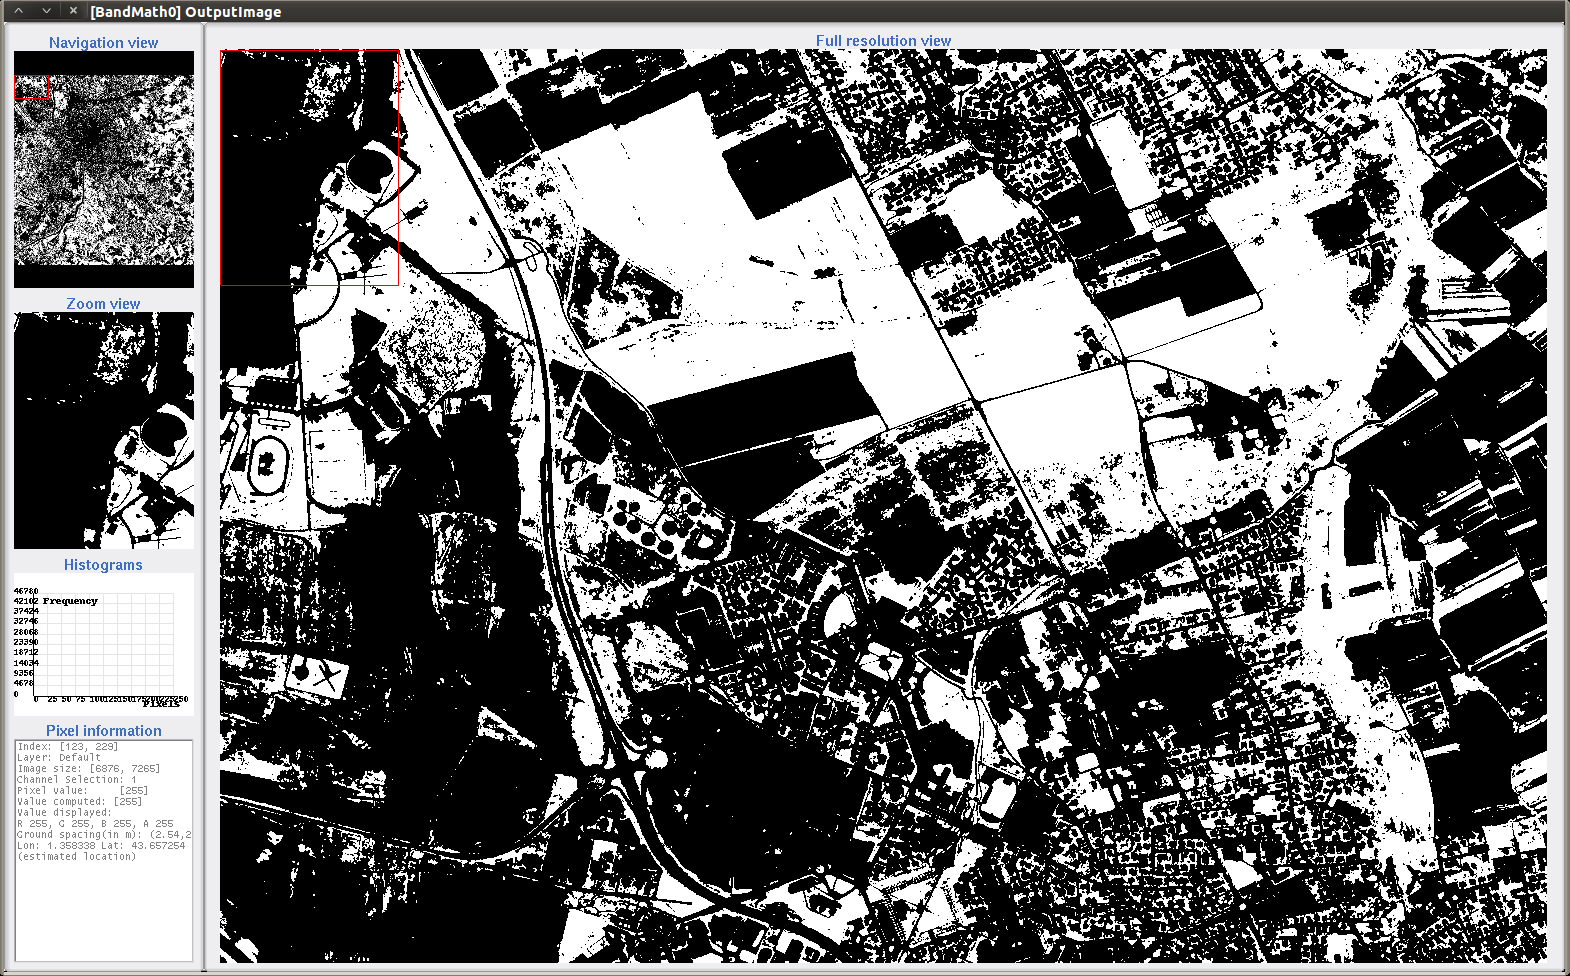
\includegraphics[width=0.6\textwidth]{../Art/MonteverdiImages/monteverdi_band_math_result.png}
  \itkcaption[Result of Band math operations module]{NDVI image threshold.}
  \label{fig:bandmathresult}
\end{figure}

\begin{figure}
  \center
  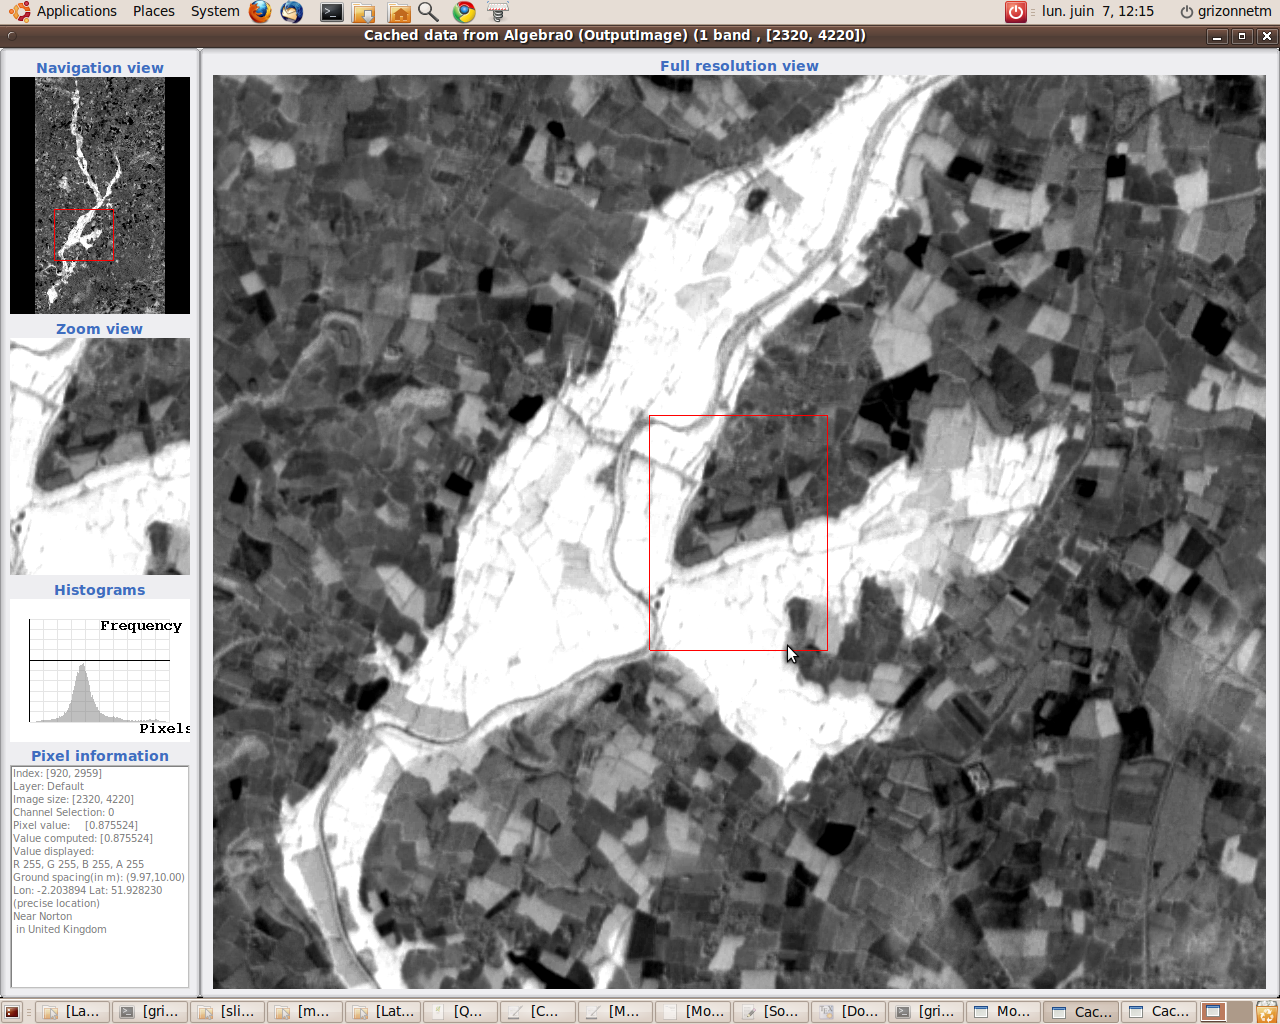
\includegraphics[width=0.6\textwidth]{../Art/MonteverdiImages/monteverdi_NDWI2_substraction.png}
  \itkcaption[Difference of NDWI2 on 2 images]{Subtraction of NDWI2.}
  \label{fig:ndwi2}
\end{figure}

\subsubsection{Feature extraction}

Under the term Feature Extraction, it include several techniques
aiming to detect or extract infor- mations of low level of abstraction
from images. These features can be objects : points, lines, etc.They
can also be measures : moments, textures, etc.

\subsubsection{Mean-shift segmentation}

For a given pixel, the Mean-shift algorithm will build a set of
neighboring pixels within a given spatial radius and a color
range. The spatial and color center of this set is then computed and
the algorithm iterates with this new spatial and color center. The
Mean-shift can be used for edge-preserving smoothing, or for
clustering.

\begin{figure}
  \center
  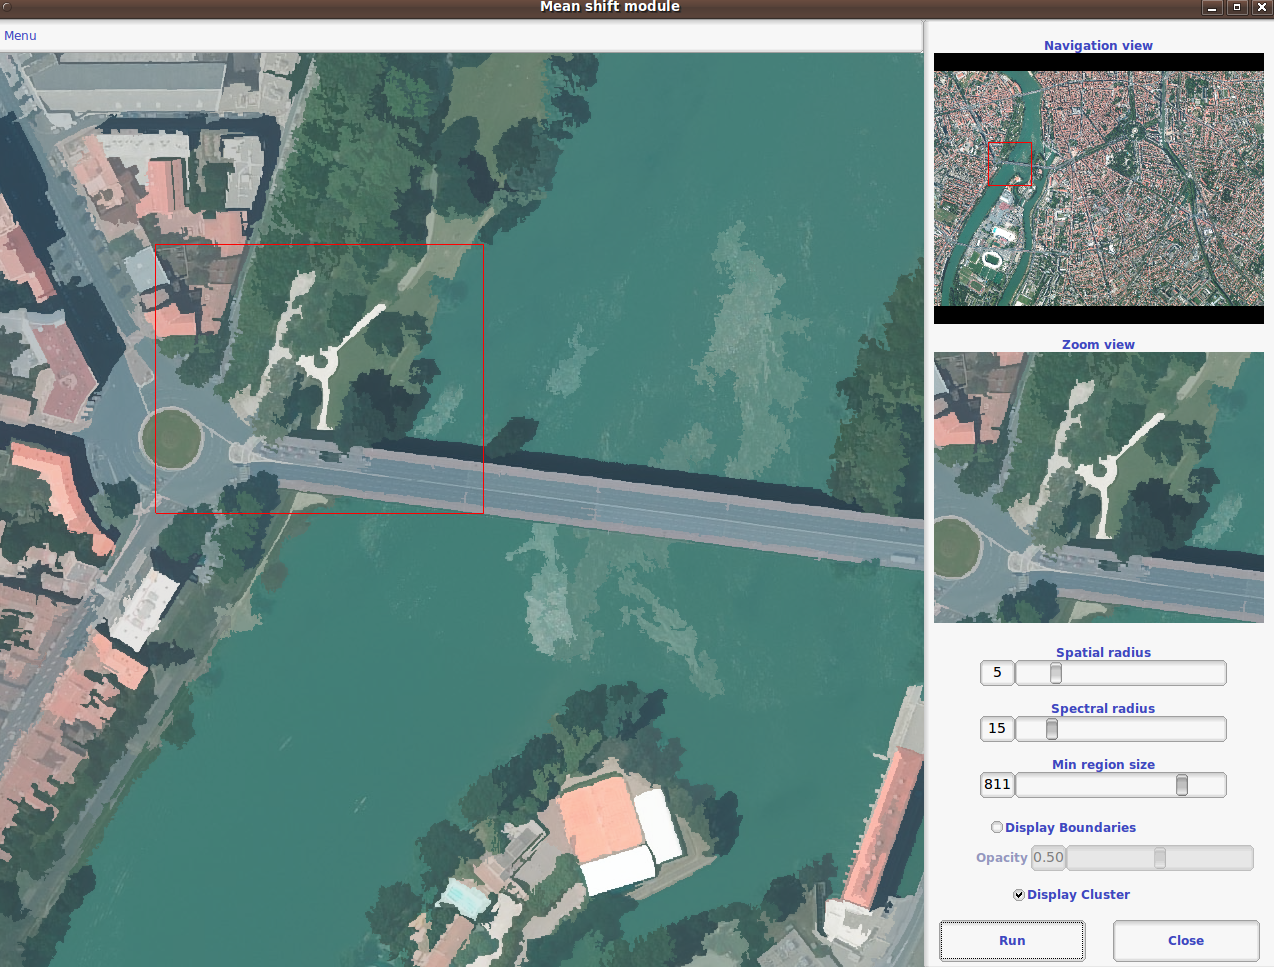
\includegraphics[width=0.6\textwidth]{../Art/MonteverdiImages/monteverdi_mean_shift.png}
  \itkcaption[Mean-shift clustering]{Mean-shift module.}
  \label{fig:meanshift}
\end{figure}

\subsection{Learning}
\subsubsection{Supervised classification}
Supervised classification is a procedure in which individual items are
placed into groups based on quantitative information on one or more
characteristics inherent in the items and based on a training set of
previously labeled items.

The supervised classification module is based on the Support Vector
Machine method which consists in searching for the separating surface
between 2 classes by the determination of the subset of training
samples which best describes the boundary between the 2 classes. This
method can be extended to be able to classify more than 2 classes.

The module allows to interactivelly describe learnings samples which
corresponds to polygons samples on the input images.

Then a SVM model is derived from this learning sample which allows to
classify each pixel of the input image in one of the defined class.


\subsubsection{Non-supervised classification}
The non supervised classification module is based on the Kmeans
algorithm.  The GUI allows to modify parameters of the algorithm and
produce a label image.
\subsection{Specific SAR functionnalities}
This section give access to specific treatments related to the SAR
functionnalities

\begin{itemize}
\item Synthetic aperture radar images are generally corrupted by
  speckle noise.  To suppress speckle and improve the radar image
  interpretability lots of filtering techniques have been proposed.
  The module implements to well-known despeckle methods: Frost and
  Lee.
\item Derived intensity and log-intensity from the input SAR imagery.
\item Polarization Synthesis : Allow to construct an image that would
  be received from a polarimetric radar having selected transmit and
  receive polarizations.
\end{itemize}
